\documentclass[]{book}
\usepackage{lmodern}
\usepackage{amssymb,amsmath}
\usepackage{ifxetex,ifluatex}
\usepackage{fixltx2e} % provides \textsubscript
\ifnum 0\ifxetex 1\fi\ifluatex 1\fi=0 % if pdftex
  \usepackage[T1]{fontenc}
  \usepackage[utf8]{inputenc}
\else % if luatex or xelatex
  \ifxetex
    \usepackage{mathspec}
  \else
    \usepackage{fontspec}
  \fi
  \defaultfontfeatures{Ligatures=TeX,Scale=MatchLowercase}
\fi
% use upquote if available, for straight quotes in verbatim environments
\IfFileExists{upquote.sty}{\usepackage{upquote}}{}
% use microtype if available
\IfFileExists{microtype.sty}{%
\usepackage[]{microtype}
\UseMicrotypeSet[protrusion]{basicmath} % disable protrusion for tt fonts
}{}
\PassOptionsToPackage{hyphens}{url} % url is loaded by hyperref
\usepackage[unicode=true]{hyperref}
\hypersetup{
            pdfborder={0 0 0},
            breaklinks=true}
\urlstyle{same}  % don't use monospace font for urls
\usepackage{graphicx,grffile}
\makeatletter
\def\maxwidth{\ifdim\Gin@nat@width>\linewidth\linewidth\else\Gin@nat@width\fi}
\def\maxheight{\ifdim\Gin@nat@height>\textheight\textheight\else\Gin@nat@height\fi}
\makeatother
% Scale images if necessary, so that they will not overflow the page
% margins by default, and it is still possible to overwrite the defaults
% using explicit options in \includegraphics[width, height, ...]{}
\setkeys{Gin}{width=\maxwidth,height=\maxheight,keepaspectratio}
\IfFileExists{parskip.sty}{%
\usepackage{parskip}
}{% else
\setlength{\parindent}{0pt}
\setlength{\parskip}{6pt plus 2pt minus 1pt}
}
\setlength{\emergencystretch}{3em}  % prevent overfull lines
\providecommand{\tightlist}{%
  \setlength{\itemsep}{0pt}\setlength{\parskip}{0pt}}
\setcounter{secnumdepth}{0}
% Redefines (sub)paragraphs to behave more like sections
\ifx\paragraph\undefined\else
\let\oldparagraph\paragraph
\renewcommand{\paragraph}[1]{\oldparagraph{#1}\mbox{}}
\fi
\ifx\subparagraph\undefined\else
\let\oldsubparagraph\subparagraph
\renewcommand{\subparagraph}[1]{\oldsubparagraph{#1}\mbox{}}
\fi

% set default figure placement to htbp
\makeatletter
\def\fps@figure{htbp}
\makeatother


\date{}

\begin{document}

\begin{itemize}
\tightlist
\item
  \protect\hyperlink{page1}{Installation}

  \begin{itemize}
  \tightlist
  \item
    \protect\hyperlink{part1}{Composer}
  \item
    \protect\hyperlink{part2}{Einrichtung}
  \end{itemize}
\item
  \protect\hyperlink{page2}{Konfiguration}

  \begin{itemize}
  \tightlist
  \item
    \protect\hyperlink{part3}{Statisches Typoscript inkludieren}
  \item
    \protect\hyperlink{part4}{Konstanten für die SOLR Connection
    einrichten}
  \item
    \protect\hyperlink{part5}{Search Marker}
  \item
    \protect\hyperlink{part6}{Indexierung aktivieren}
  \item
    \protect\hyperlink{part7}{Root-Page definieren}
  \item
    \protect\hyperlink{part8}{SOLR Connections intialisieren}
  \item
    \protect\hyperlink{part9}{Verbindungen überprüfen}
  \end{itemize}
\item
  \protect\hyperlink{page3}{Indexierung}

  \begin{itemize}
  \tightlist
  \item
    \protect\hyperlink{part10}{Inhalte für Indexierung wählen}
  \item
    \protect\hyperlink{part11}{Scheduler Tasks einrichten}
  \end{itemize}
\item
  \protect\hyperlink{page4}{Anzeige der Suche und Ergebnisse}

  \begin{itemize}
  \tightlist
  \item
    \protect\hyperlink{part12}{Seite anlegen}
  \item
    \protect\hyperlink{part13}{Content Element einfügen}
  \item
    \protect\hyperlink{part14}{Suchen}
  \end{itemize}
\item
  \protect\hyperlink{page5}{Anpassung}

  \begin{itemize}
  \item
    \protect\hyperlink{part15}{Anpassung der Templates in Version 7}

    \chapter{Installation}
  \end{itemize}
\end{itemize}

\section{Composer}

Wechsele in das TYPO3 Verzeichnis und installiere die Extension SOLR mit
folgendem Befehl:

\section{Einrichtung}

\begin{itemize}
\tightlist
\item
  Wechsele in den Bereich ``Extensions''

  \begin{itemize}
  \tightlist
  \item
    Gebe bei Suche ``solr'' ein
  \item
    Aktiviere die Extension
  \end{itemize}
\end{itemize}

\chapter{Konfiguration}

\section{Statisches Typoscript inkludieren}

\begin{itemize}
\tightlist
\item
  Wechsele in den Bereich ``Template'' und wähle den obersten Knoten der
  Webseite aus

  \begin{itemize}
  \tightlist
  \item
    Wähle ``Info/Modify'' im Dropdown aus
  \item
    Wähle ``Edit the whole template record''
  \item
    Wähle im Menü ``Includes''
  \item
    Klicke rechts auf die Option ``Search - Base Configuration (solr)''
    und füge sie hinzu
  \item
    Klicke auf ``Save'' um die Einstellungen zu speichern
  \end{itemize}
\end{itemize}

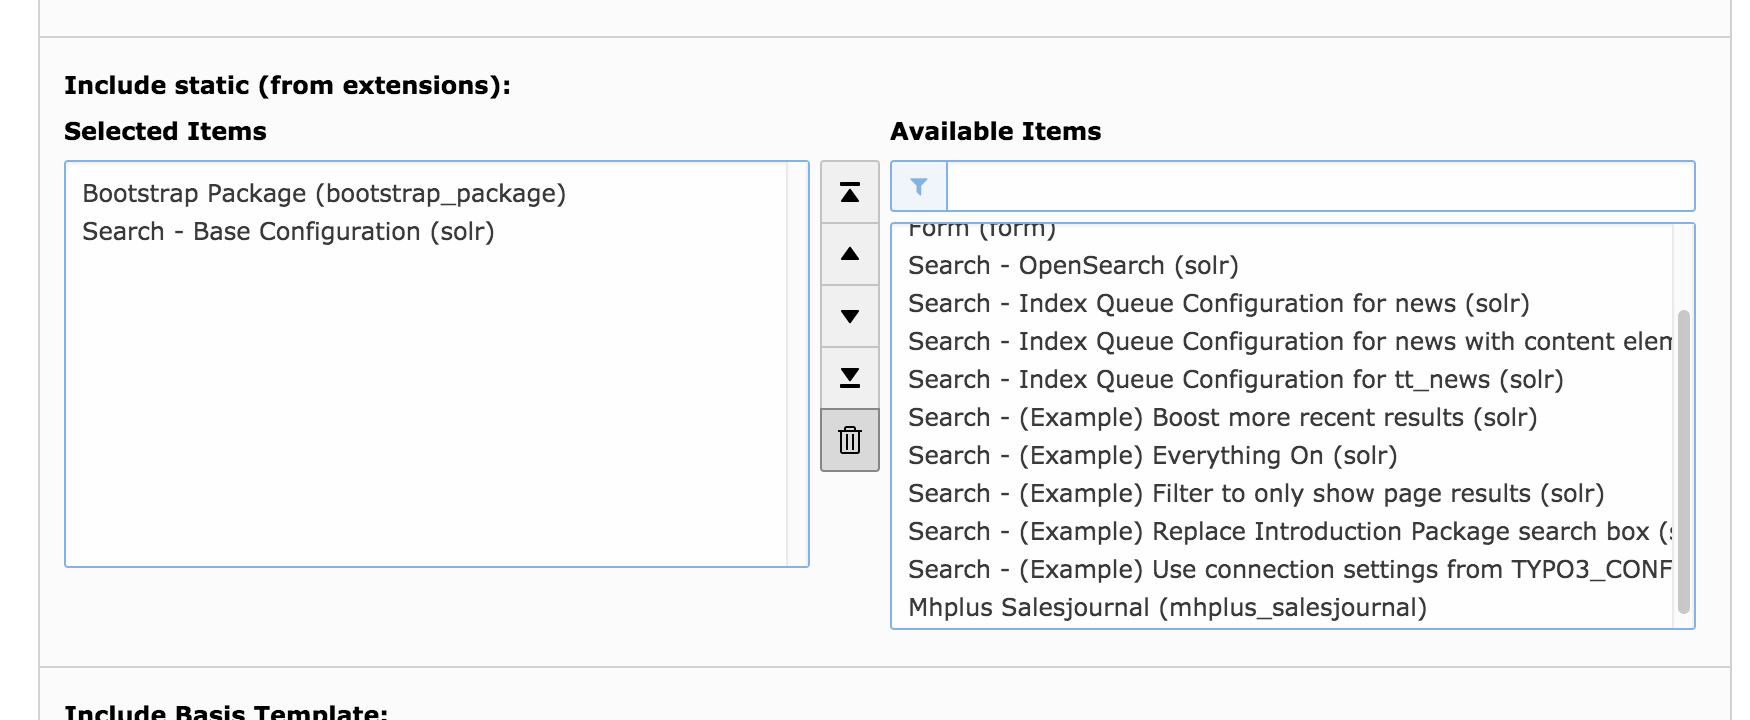
\includegraphics{images/static_typoscript.png}

\section{Konstanten für die SOLR Connection einrichten}

Aktualisiere die Konstanten auf Deiner Root-Page mit folgendem
Typoscript:

Denke daran, den Wert für host anzupassen, wenn SOLR auf einem externen
Server läuft.

\section{Search Marker}

EXR:solr indexiert alles zwischen

Sollten diese Marker nicht vorhanden sein, müssen diese hinzugefügt
werden. Vor allem um die Qualität zu erhöhen und nur die relevanten
Inhalte zu indexieren. Der einfachste Weg ist, dies mit Typoscript zu
tun:

\section{Indexierung aktivieren}

Das Indexing wird mit folgendem Tyoscript aktiviert:

\section{Root-Page definieren}

Wichtig ist auch, dass die Root-Page als solche aktiviert ist.

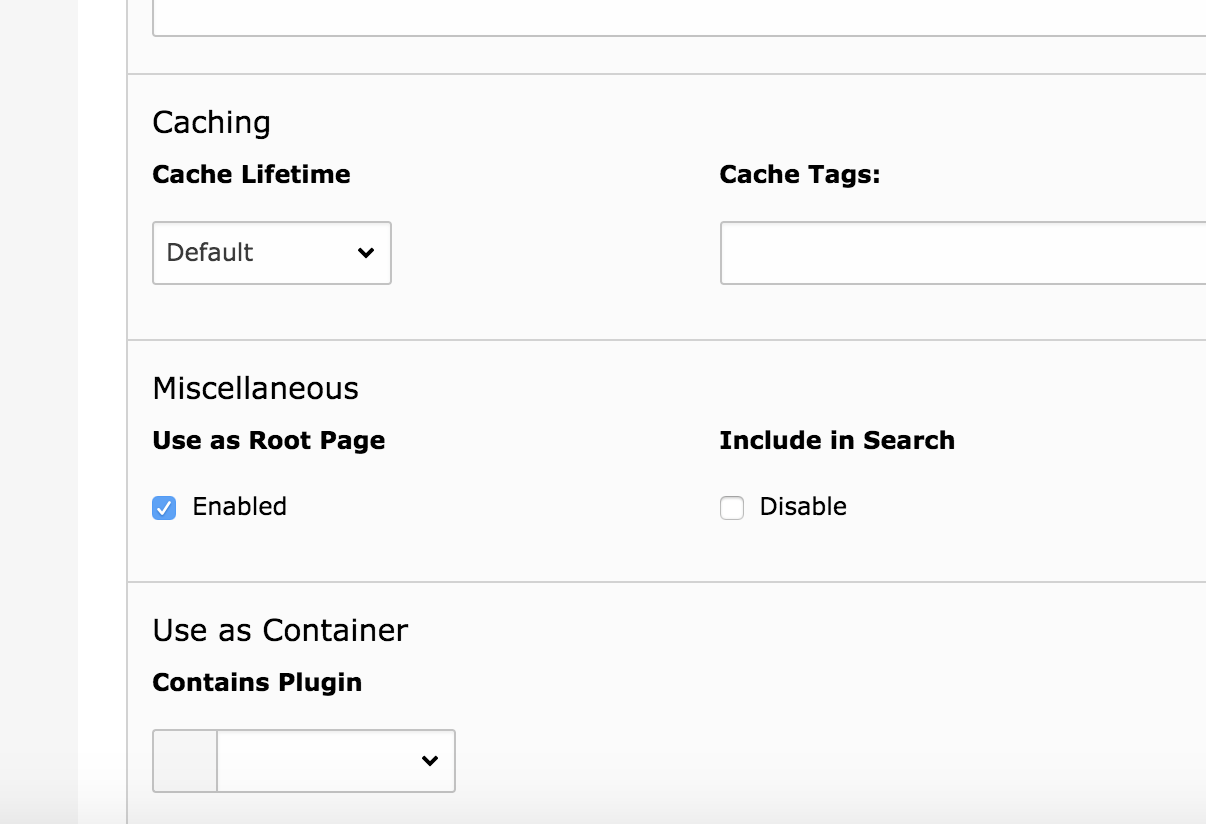
\includegraphics{images/root_page.png}

\begin{itemize}
\tightlist
\item
  Aktviere die Checkbox bei \textbf{Use as Root Page}
\end{itemize}

\section{SOLR Connections intialisieren}

Als nächstes müssen die SOLR Connections aktiviert werden. Zum
Initialisieren wähle aus dem Menü ``Initialize Solr connections'':

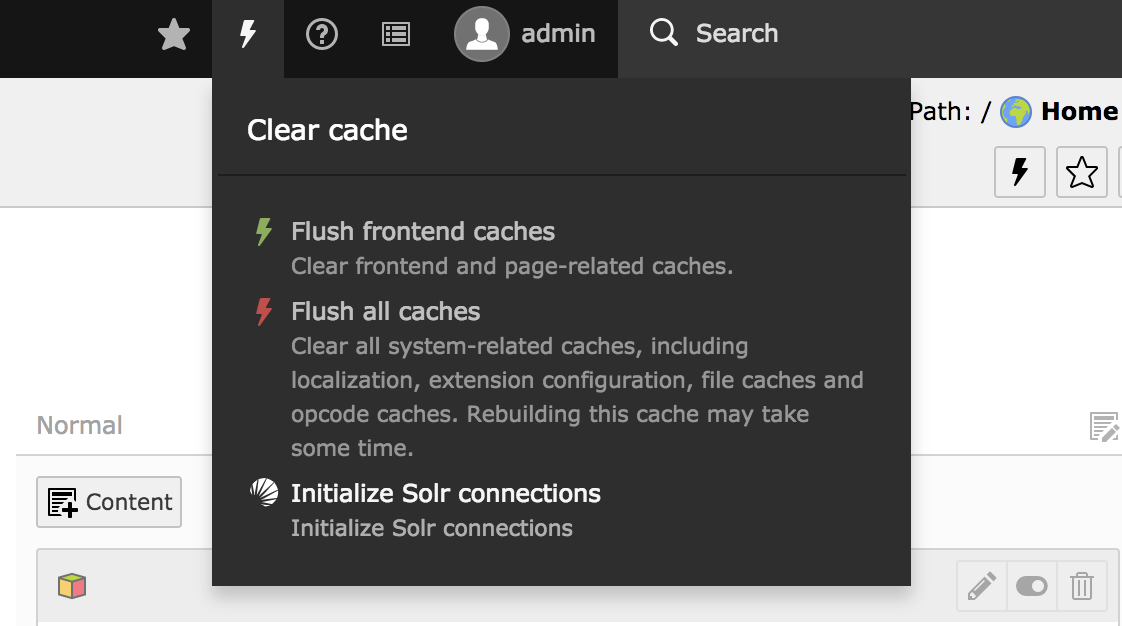
\includegraphics{images/solr_connection.png}

\section{Verbindungen überprüfen}

\begin{itemize}
\tightlist
\item
  Gehe zu ``Reports''
\item
  Schaue Dir an ob bei ``solr'' Fehlermeldungen aufgetreten sind und ob
  die Verbindung geklappt hat
\end{itemize}

\chapter{Indexierung}

\section{Inhalte für Indexierung wählen}

Wenn alles eingerichtet ist, wechsele auf der linken Seite zum Menüpunkt
``Search''. Klicke im Modul auf ``Index Queue'', wähle die Inhalte aus
und klicke auf ``Queue selected content for indexing''.

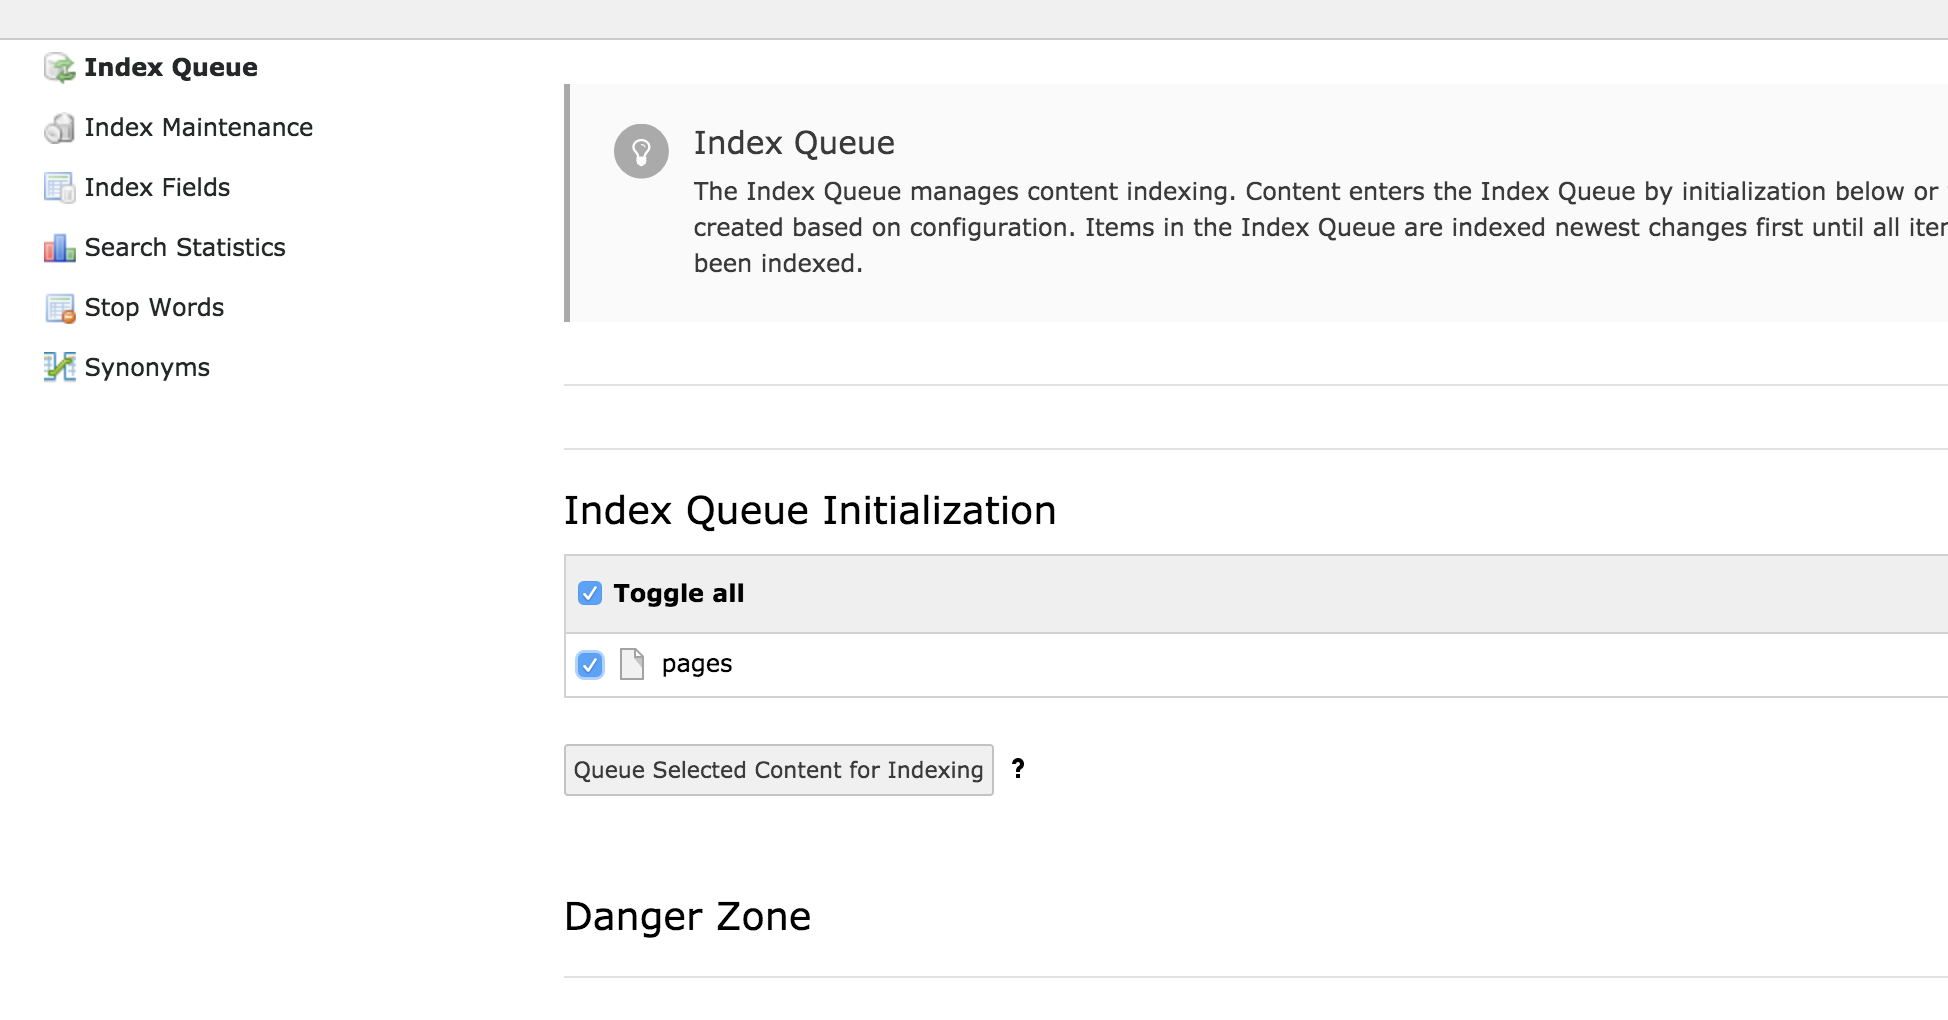
\includegraphics{images/queue.png}

\section{Scheduler Tasks einrichten}

Damit die Indexierung tatsächlich durchgeführt wird, muss ein Scheduler
Task eingerichtet werden, der auch manuell ausgeführt werden kann.

\begin{itemize}
\tightlist
\item
  Wähle ``Scheduler''
\item
  Füge einen neuen Task hinzu
\item
  Wähle aus der Oberkategorie solr den task ``Index Queue Worker'' aus
\item
  Klicke auf Speichern, damit wird der Task angelegt
\item
  Klicke in der Übersicht der Scheduler beim entsprechenden Task auf das
  play Symbol und ``Run task''
\end{itemize}

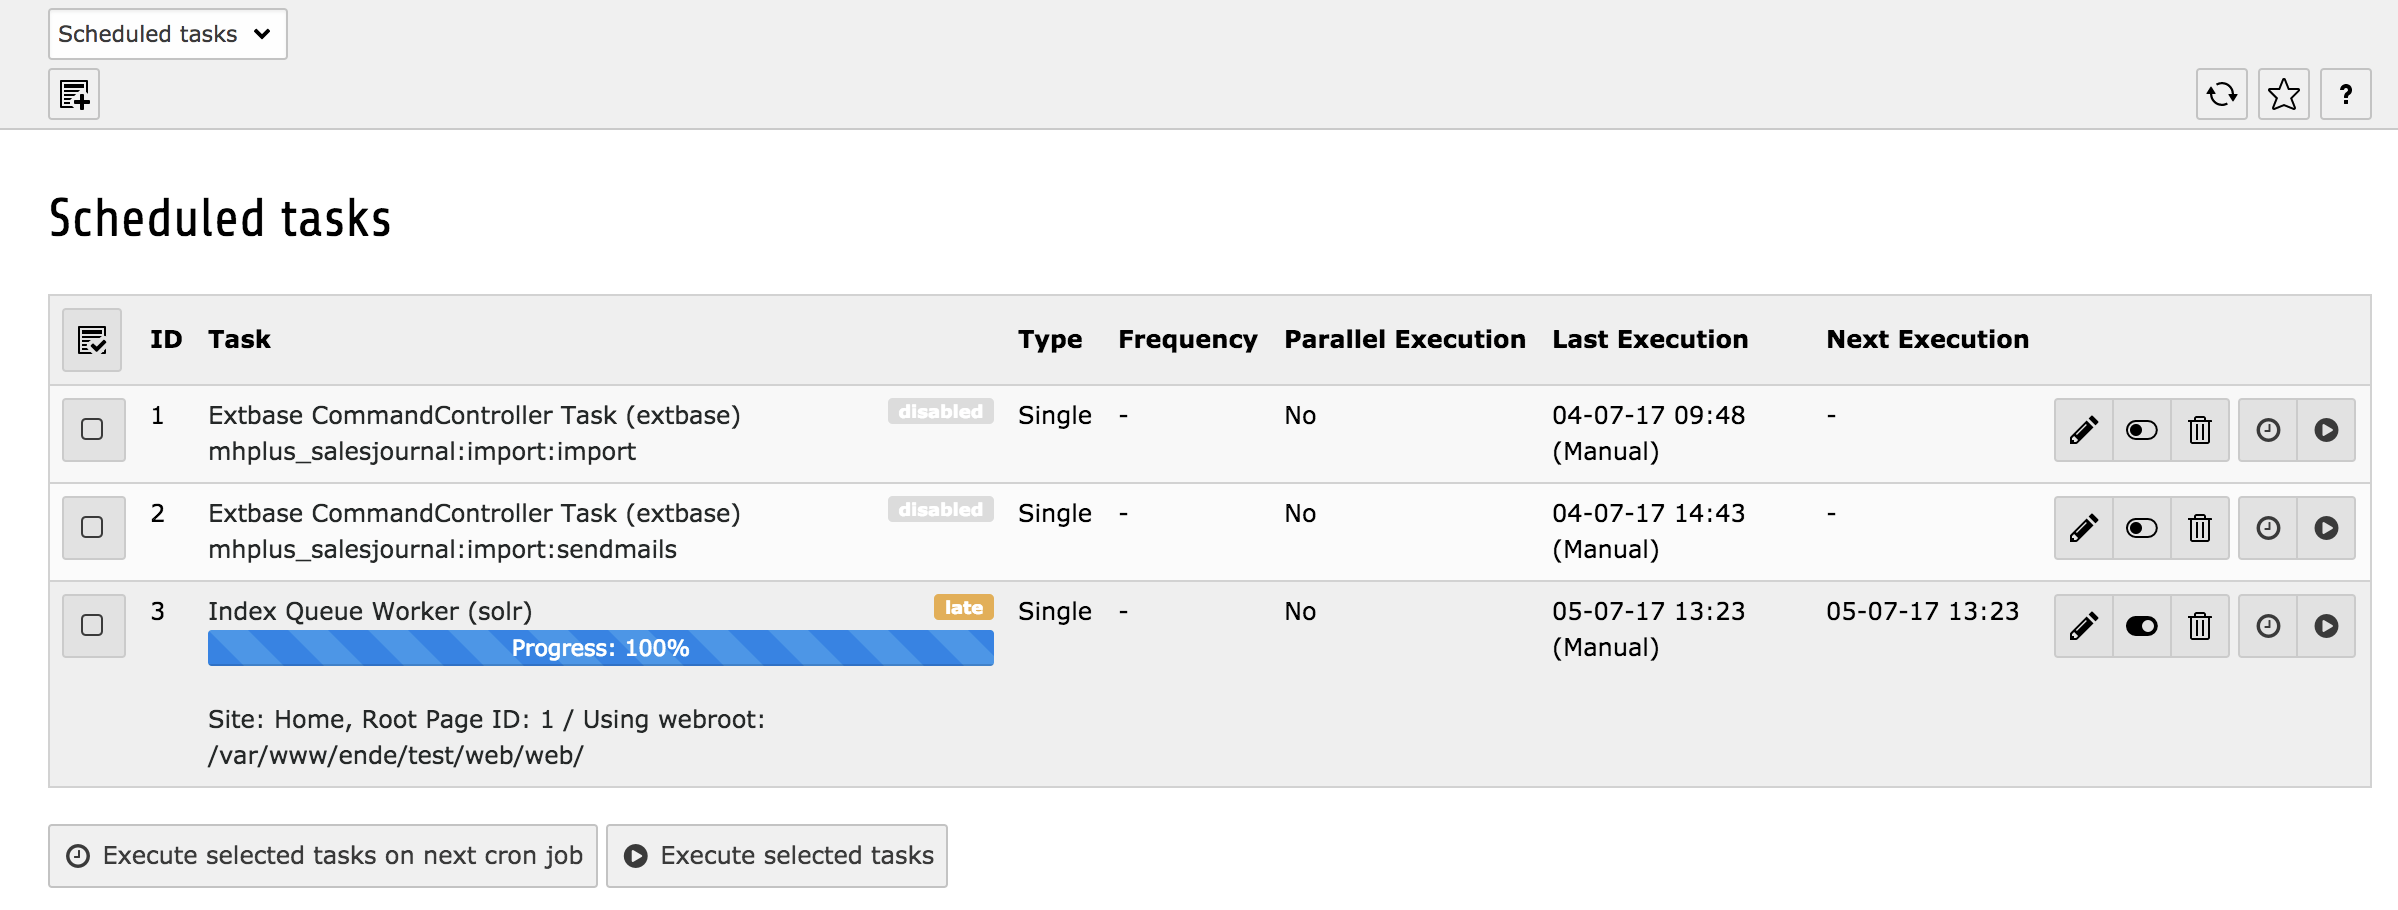
\includegraphics{images/scheduler.png}

\chapter{Anzeige der Suche und Ergebnisse}

\section{Seite anlegen}

Lege unterhalb des Page Roots eine Seite ``Suche'' an.

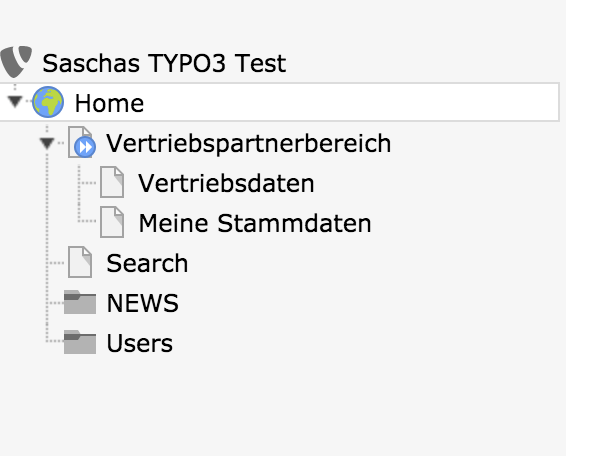
\includegraphics{images/searchpage.png}

\section{Content Element einfügen}

Füge das Plugin ``Search'' auf der Seite ein.

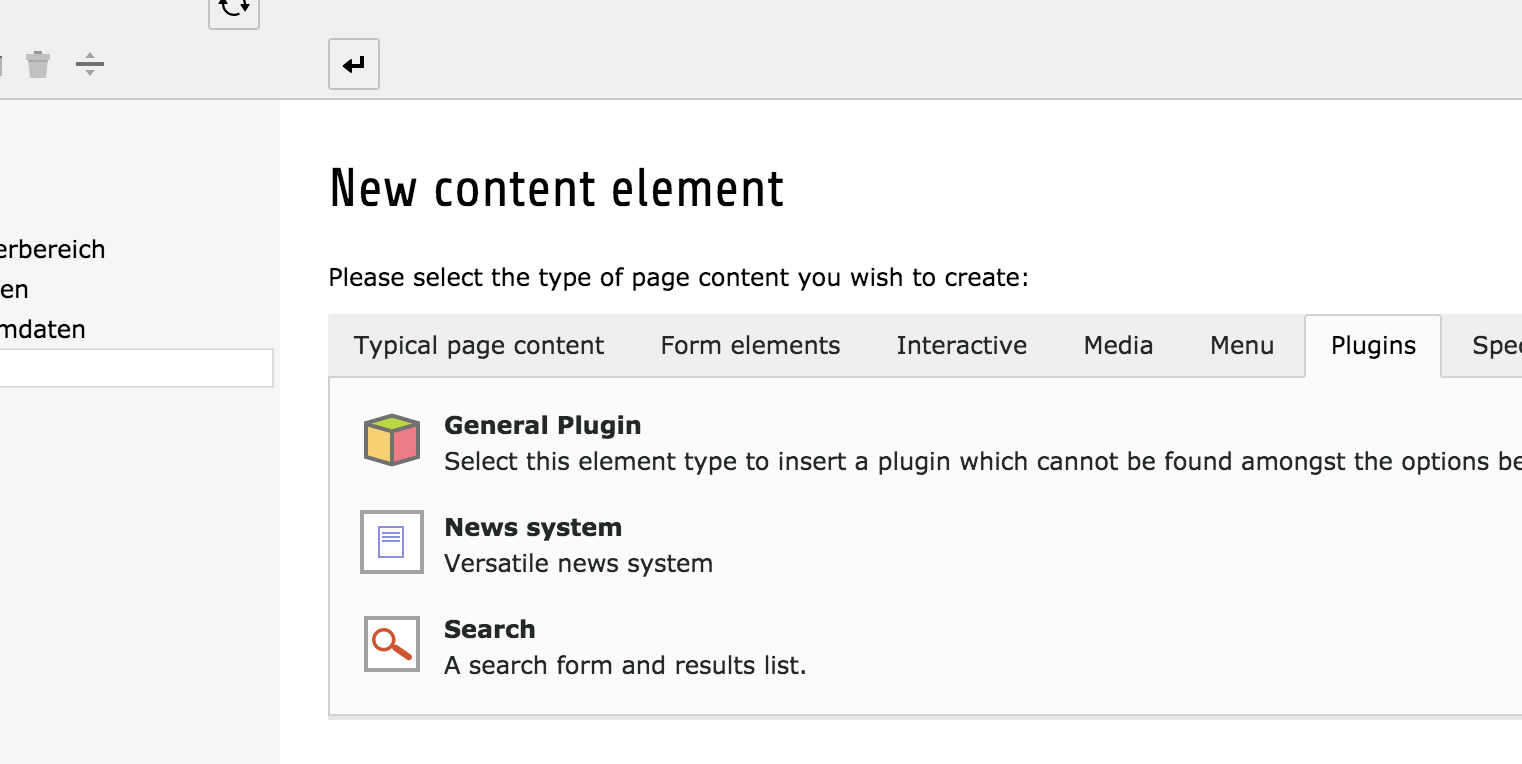
\includegraphics{images/add_plugin.png}

\section{Suchen}

Öffne die Seite ``Suche'' auf der Webseite und gebe ``*" ein. Du
solltest nun die ersten Inhalte sehen.

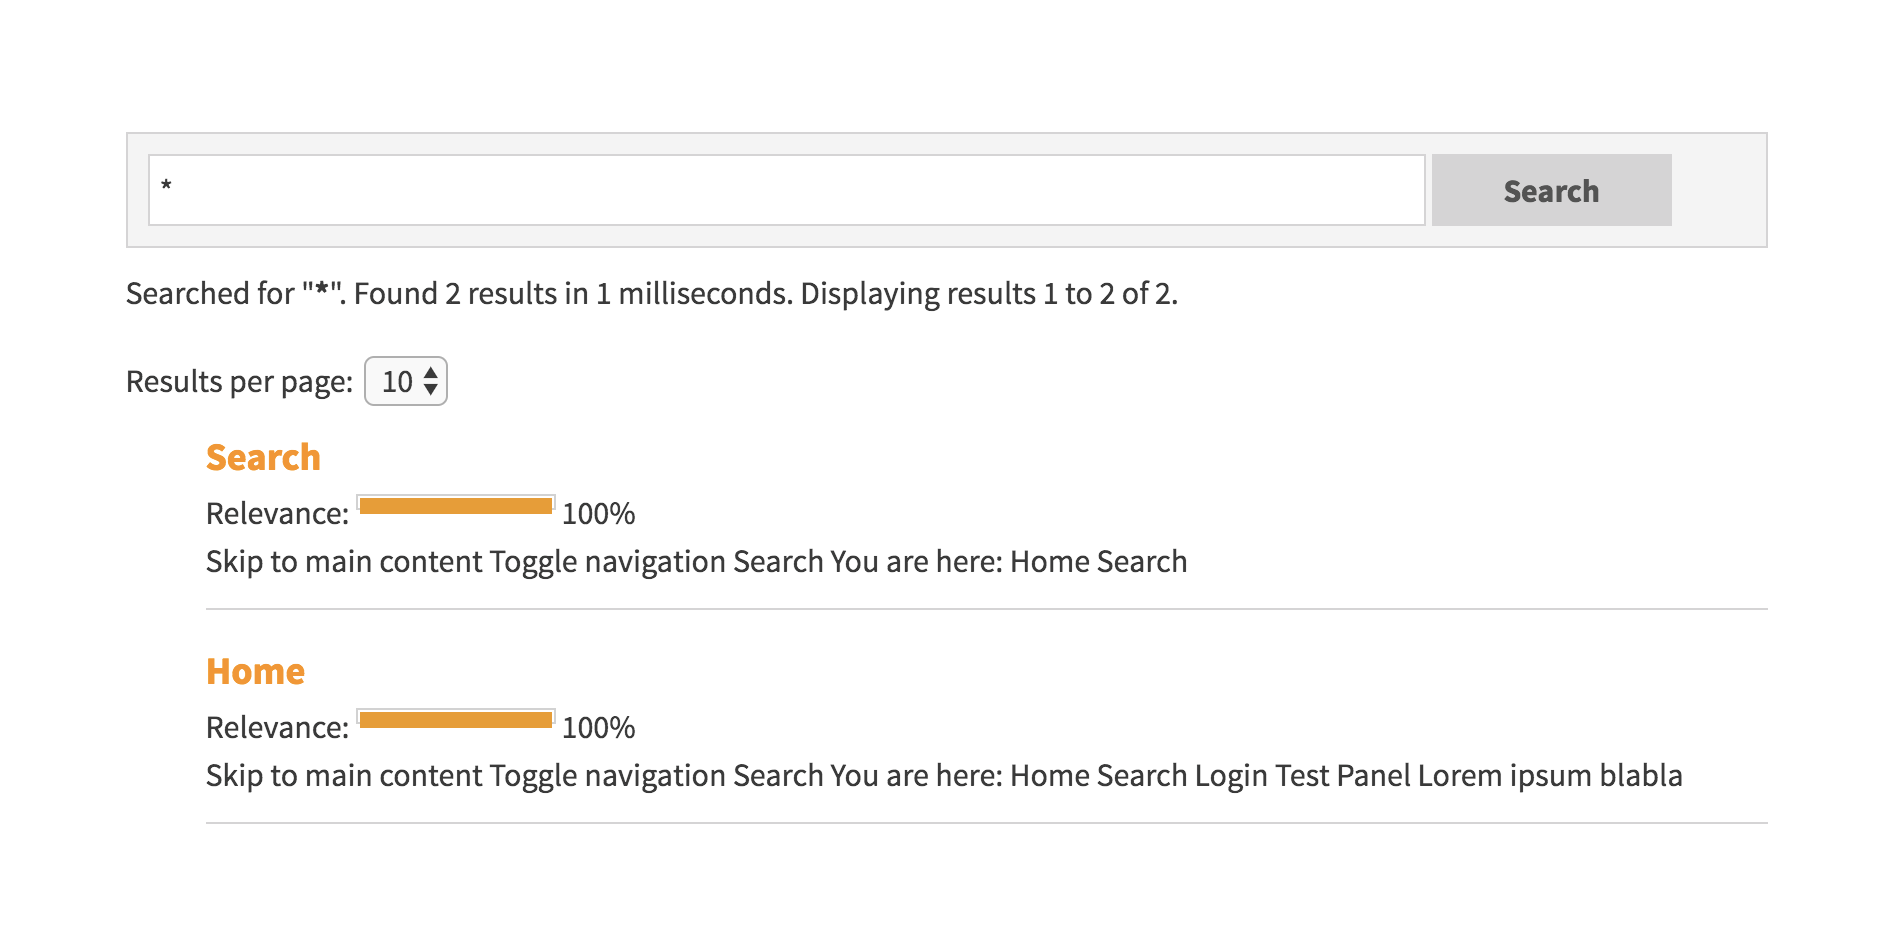
\includegraphics{images/searchresults.png}

\chapter{Anpassung}

\section{Anpassung der Templates in Version 7}

Der Pfad zu den Templates kann über folgendes Typoscript angepasst
werden. Der entsprechende Vermerk dazu findet sich auch in
\textbf{Configuration/TypoScript/Solr/setup.txt}

\end{document}
